%Disciplina Projetos de Automação
%Turma: Engenharia de software
%Integrantes do grupo:
%Anna Lívia Vasconcelhos, Gabriel Dias, Lucas Sanches Marcilio, Mirella Costa Viana e Thalyson Gama da Costa

\documentclass[10pt]{article}  
\usepackage[portuguese]{babel} 
\usepackage[utf8]{inputenc} % Indica que a codificação é utf8  
\usepackage{amsmath} % Comandos extras para matemática
\usepackage{amssymb} % Símbolos matemáticos
\usepackage{graphicx} % Incluir imagens no LaTeX
\usepackage{color} % Para colorir texto
\usepackage{subfigure} % subfiguras
\usepackage{float} % Podemos usar o especificador [H] nas figuras para que fiquem na posição desejada
\usepackage{capt-of} % Permite usar etiquetas fora de elementos flutuantes
\usepackage{sidecap} % Para colocar o texto das imagens ao lado delas
	\sidecaptionvpos{figure}{c} 
\usepackage{caption} % Para poder colocar a numeração nas figuras
\usepackage{anysize}% Para personalizar os tamanhos das margens
	\marginsize{2cm}{2cm}{2cm}{2cm} % Esquerda, direita, acima, abaixo
\usepackage{appendix}
	\renewcommand{\appendixname}{Apêndices}
	\renewcommand{\appendixtocname}{Apêndices}
	\renewcommand{\appendixpagename}{Apêndices} 
\usepackage[colorlinks=true,plainpages=true,citecolor=blue,linkcolor=blue]{hyperref} 
\usepackage{fancyhdr} 
	\pagestyle{fancy}
	\fancyhf{}
	\fancyhead[L]{\footnotesize UNISAL - CENTRO SALESIANO DE SÃO PAULO} % Cabeçalho à esquerda
	\fancyhead[R]{\footnotesize Engenharia de Software}   % Cabeçalho à direita
	\fancyfoot[R]{\footnotesize Documentação}  % Rodapé à direita
	\fancyfoot[C]{\thepage}  
	\fancyfoot[L]{\footnotesize Automação Industrial} 
	\renewcommand{\footrulewidth}{0.4pt}
\usepackage{listings} 
\usepackage{tcolorbox}
\usepackage{enumitem}

\definecolor{codebg}{RGB}{245,245,245}
\definecolor{codeframe}{RGB}{210,210,210}
\definecolor{keyword}{RGB}{0,102,102}
\definecolor{comment}{RGB}{120,120,120}
\definecolor{string}{RGB}{170,55,55}

\lstdefinestyle{plantuml}{
    backgroundcolor=\color{codebg},
    basicstyle=\ttfamily\small,
    frame=single,
    rulecolor=\color{codeframe},
    breaklines=true,
    captionpos=b,
    keywordstyle=\color{keyword}\bfseries,
    commentstyle=\color{comment}\itshape,
    stringstyle=\color{string},
    showstringspaces=false,
    keywords={class,interface,abstract,enum,package,extends,implements}
}

\lstset{style=plantuml}

\newtcolorbox{destaque}[1]{
    colback=teal!5,
    colframe=teal!50!black,
    fonttitle=\bfseries,
    title=#1,
    boxrule=0.5pt,
    arc=2pt
}

\title{Documento Arquitetural}

\begin{document}
\begin{center}														
\newcommand{\HRule}{\rule{\linewidth}{0.5mm}} 

\begin{minipage}{0.48\textwidth} \begin{center}
	
\includegraphics[scale = 0.54]{Imagens/logo_light.png}
\end{center}
\end{minipage}

\vspace*{1.5cm} 
\textsc{\huge Sistema de gestão de\\ \vspace{5px}  Falhas Industriais}\\[1.5cm]	
\textsc{\LARGE Disciplina: Engenharia de Software }\\[1.5cm]									
\vspace*{1.5cm}																	
\HRule \\[0.5cm]
{ \Huge \bfseries Documento Arquitetural }\\[0.2cm]
{ \huge \bfseries Refatoração com Padrões de Projeto (GoF)} 													
\HRule \\[1.5cm]																

\begin{minipage}{0.46\textwidth}
	\begin{flushleft} \large
		\emph{Autores:}\\	
		Anna Lívia Vasconcelhos, Gabriel Dias, Lucas Sanches Marcilio, Mirella Costa Viana e Thalyson Gama da Costa
	\end{flushleft}																
\end{minipage}		
\begin{minipage}{0.52\textwidth}		
\vspace{-0.6cm}
	\begin{flushright} \large															\emph{Funções:} \\														
		Refatoração Arquitetural 
	\end{flushright}															
\end{minipage}	
\vspace*{1cm}
\vspace{2cm} 																				
\begin{center}																		{v1.0.0 - 02 de junho de 2026}
\end{center}												 					
\end{center}							 																									
\newpage

\textbf{\Huge Resumo} 
\\
\linebreak
Este documento descreve a refatoração do diagrama de classes do
Sistema de Gestão de Falhas de Manutenção Industrial mediante a aplicação de
cinco padrões de projeto do catálogo \textit{Gang of Four} (GoF). Para cada
padrão são apresentados: o problema identificado no projeto original, a solução
proposta, a justificativa técnica, o impacto arquitetural, as vantagens e
limitações, e o trecho atualizado do diagrama de classes em imagens. Os
padrões escolhidos --- \textbf{State}, \textbf{Strategy}, \textbf{Observer},
\textbf{Factory Method} e \textbf{Facade} --- cobrem as três categorias do
catálogo (comportamental, criacional e estrutural). Por restrição do trabalho,
não foram utilizados os padrões \textit{Abstract Factory}, \textit{Adapter} e
\textit{Decorator}.

\newpage
\tableofcontents  

\newpage
\section{Visão Geral da Refatoração}

O diagrama original concentrava grande quantidade de responsabilidades na classe
\texttt{Falha} e utilizava enumerações (\texttt{StatusChamada},
\texttt{Prioridade}) carregadas de regras de negócio implícitas. A criação dos
diversos subtipos de \texttt{Funcionario} ocorria de forma direta, e a
orquestração do fluxo de atendimento ficava a cargo do cliente. Esses pontos
representavam \textit{code smells} clássicos: classe inchada, condicionais
espalhados, alto acoplamento e baixa coesão.

A Tabela~\ref{tab:padroes} resume os cinco padrões aplicados e o
\textit{smell} que cada um resolve.

\begin{table}[h]
\centering
\begin{tabular}{|l|l|p{7cm}|}
\hline
\textbf{Padrão} & \textbf{Categoria} & \textbf{Problema que resolve} \\
\hline
State & Comportamental & Transições de \texttt{statusChamada} controladas por condicionais espalhados. \\
\hline
Strategy & Comportamental & Regra fixa e rígida de priorização dentro de \texttt{Falha}. \\
\hline
Observer & Comportamental & Acoplamento direto entre \texttt{Falha} e os serviços de alerta/notificação. \\
\hline
Factory Method & Criacional & Instanciação direta (\texttt{new}) dos subtipos de \texttt{Funcionario}. \\
\hline
Facade & Estrutural & Cliente obrigado a orquestrar múltiplos objetos do subsistema. \\
\hline
\end{tabular}
\caption{Padrões aplicados e respectivos problemas.}
\label{tab:padroes}
\end{table}

\begin{destaque}{Por que estes cinco padrões?}
A escolha priorizou padrões que eliminam dores reais já presentes no diagrama,
e não padrões ``encaixados à força''. Cada padrão remove um acoplamento ou uma
rigidez específica, e o conjunto cobre as três categorias do catálogo GoF,
demonstrando domínio das diferentes intenções de projeto.
\end{destaque}

\newpage

% ==================================================================
\section{Padrão State (Comportamental)}

\subsection{Problema identificado}
A classe \texttt{Falha} possuía o atributo \texttt{statusChamada} do tipo
enumeração. Toda regra de transição --- por exemplo, ``só é possível aprovar uma
falha que esteja em análise'' --- era implementada com estruturas
condicionais (\texttt{if/switch}) espalhadas pelos métodos \texttt{aprovar()},
\texttt{recusar()} e \texttt{concluir()}. Isso tornava o código frágil,
propenso a estados inválidos e difícil de estender.

\subsection{Solução proposta}
Cada valor do enumerado foi transformado em uma classe de estado
(\texttt{EstadoAberto}, \texttt{EstadoEmAnalise}, \texttt{EstadoAprovado}, etc.)
que implementa a interface \texttt{EstadoFalha}. Cada estado conhece apenas as
transições válidas a partir de si mesmo; transições inválidas lançam
\texttt{IllegalStateException}. A \texttt{Falha} passa a \textbf{delegar} a
operação ao estado atual.

\subsection{Justificativa técnica e por que usar}
O padrão State é a resposta canônica para objetos cujo comportamento depende de
seu estado interno. Ao distribuir a lógica de transição entre classes de estado,
elimina-se o condicional central e torna-se \textbf{impossível}, por
construção, executar uma transição inválida. A adição de um novo estado (por
exemplo, \texttt{AguardandoPeca}) não exige alterar os estados existentes,
respeitando o \textit{Open/Closed Principle}.

\subsection{Impacto arquitetural}
A responsabilidade de controle de fluxo sai da \texttt{Falha} e passa para a
hierarquia de estados, aumentando a coesão da entidade. Surge uma nova dimensão
de classes, mas cada uma é pequena e de responsabilidade única.

\subsection{Vantagens e limitações}
\begin{itemize}[leftmargin=*]
    \item \textbf{Vantagens para nosso contexto:} ajuda a elimina condicionais; transições inválidas viram
    erro explícito; fácil extensão; cada estado pode/deve ser testável isoladamente.
    \item \textbf{Limitações:} aumenta o número de classes; para máquinas de
    estado muito simples pode ser excesso de estrutura (\textit{over-engineering}).
\end{itemize}

\subsection{Trecho do diagrama de classes}
\begin{center}
		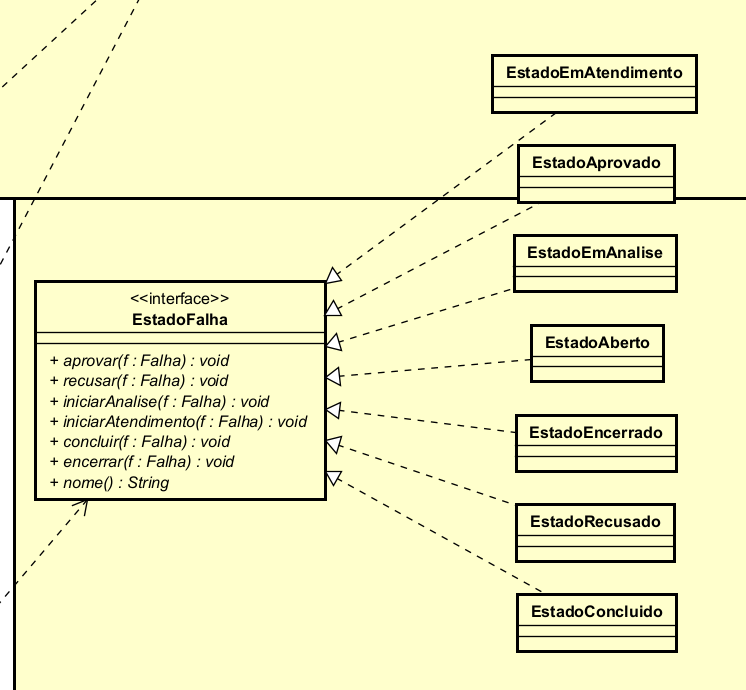
\includegraphics[width=0.8\textwidth]{Imagens/EstadoFalha.png}
		\captionof{figure}{\label{fig:diagramaState}Diagrama de Classes - Padrão State} 
	\end{center}

\newpage

% ==================================================================
\section{Padrão Strategy (Comportamental)}

\subsection{Problema identificado}
O método \texttt{aplicarPrioridadeAutomatica()} embutia uma única regra fixa de
priorização. Contudo, a priorização de falhas industriais varia conforme o
contexto: por impacto na produção, por proximidade de violação do SLA ou por
categoria. Alterar a política exigia reescrever o corpo do método dentro da
\texttt{Falha}.

\subsection{Solução proposta}
O algoritmo de priorização foi extraído para a interface
\texttt{EstrategiaPriorizacao}, com implementações intercambiáveis:
\texttt{PriorizacaoPorImpactoProducao}, \texttt{PriorizacaoPorSLA} e
\texttt{PriorizacaoPorCategoria}. A \texttt{Falha} recebe uma estratégia e
delega o cálculo a ela.

\subsection{Justificativa técnica e por que usar}
O padrão Strategy encapsula algoritmos intercambiáveis sob uma interface comum.
É a escolha correta quando existem várias formas de executar uma mesma operação
e deseja-se trocá-las sem modificar o cliente. Respeita o
\textit{Open/Closed Principle} e favorece a testabilidade, pois a estratégia
pode ser substituída em tempo de execução.

\subsection{Impacto arquitetural}
A \texttt{Falha} deixa de conhecer detalhes do cálculo de prioridade e passa a
depender apenas da abstração. As regras de negócio de priorização ficam isoladas
em classes próprias, melhorando a manutenibilidade.

\subsection{Vantagens e limitações}
\begin{itemize}[leftmargin=*]
    \item \textbf{Vantagens:} troca de algoritmo sem alterar a \texttt{Falha};
    fácil adição de novas políticas; cada estratégia é testável de forma isolada.
    \item \textbf{Limitações:} introduz mais classes; o cliente precisa conhecer
    as estratégias disponíveis para escolher a adequada.
\end{itemize}

\subsection{Trecho do diagrama de classes}
\begin{center}
        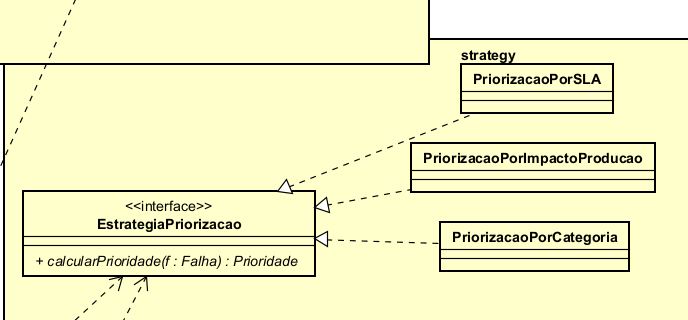
\includegraphics[width=0.8\textwidth]{Imagens/EstrategiaPriorizacao.png}
        \captionof{figure}{\label{fig:diagramaStrategy}Diagrama de Classes - Padrão Strategy} 
    \end{center}

\newpage

% ==================================================================
\section{Padrão Observer (Comportamental)}

\subsection{Problema identificado}
Quando uma falha mudava de situação, vários componentes precisavam reagir: o
\texttt{AcordoNivelServico} (SLA) verificava violações e disparava alertas, o
técnico era notificado e o painel de produção era atualizado. Se a \texttt{Falha}
chamasse cada serviço diretamente, ficaria fortemente acoplada a todos eles, e
cada novo interessado obrigaria a editar a \texttt{Falha}.
\subsection{Solução proposta}
A \texttt{Falha} tornou-se o \textit{Subject}. Os interessados implementam a
interface \texttt{ObservadorFalha} (\texttt{MonitorSLA} e
\texttt{NotificadorTecnico}, \texttt{PainelProducao}) e registram-se na falha.

Ao mudar de estado, o método \texttt{notificarObservadores()} avisa todos os
observadores sem conhecer seus tipos concretos.

\subsection{Justificativa técnica e por que usar}
O padrão Observer define uma dependência um-para-muitos de modo que, ao mudar o
estado de um objeto, todos os dependentes sejam notificados automaticamente.
É ideal quando o número de interessados é variável e não deve ser fixado em
tempo de compilação, promovendo baixo acoplamento entre emissor e receptores.

\subsection{Impacto arquitetural}
A \texttt{Falha} depende apenas da interface \texttt{ObservadorFalha}, não das
implementações. Novos observadores podem ser adicionados ou removidos em tempo
de execução, sem qualquer alteração na entidade observada.

\subsection{Vantagens e limitações}
\begin{itemize}[leftmargin=*]
    \item \textbf{Vantagens:} desacoplamento total entre \texttt{Falha} e os
    serviços reativos; registro dinâmico de observadores; aderência ao princípio
    da inversão de dependência.
    \item \textbf{Limitações:} a ordem de notificação não é garantida; em caso de
    muitos observadores, pode haver impacto de desempenho ou notificações em
    cascata difíceis de depurar.
\end{itemize}

\subsection{Trecho do diagrama de classes}
\begin{center}
        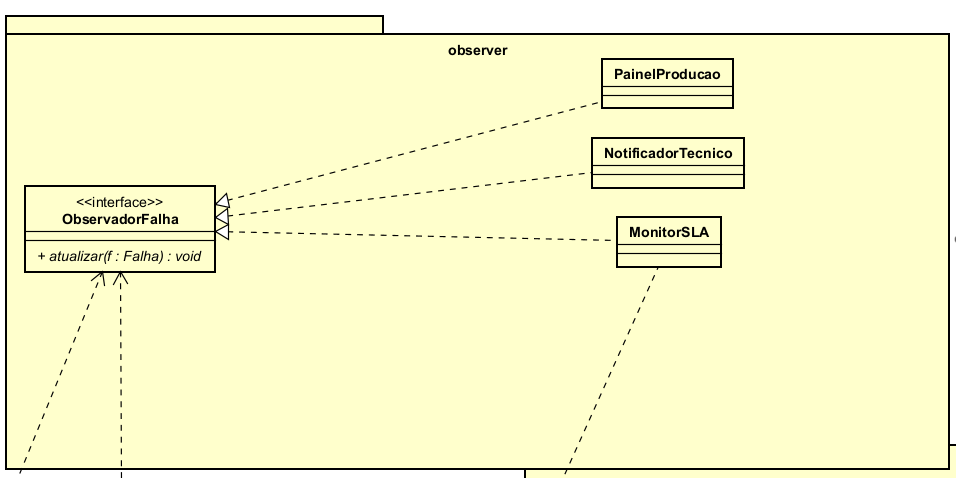
\includegraphics[width=0.8\textwidth]{Imagens/observer.png}
        \captionof{figure}{\label{fig:diagramaObserver}Diagrama de Classes - Padrão Observer} 
    \end{center}

\newpage

% ==================================================================
\section{Padrão Factory Method (Criacional)}

\subsection{Problema identificado}
O sistema possui diversos subtipos de \texttt{Funcionario} (\texttt{Tecnico},
\texttt{Operador}, \texttt{Gerente}, entre outros). A criação direta com
\texttt{new} espalhava pelo código a lógica comum de inicialização (definir
\texttt{status = ATIVO}, validar matrícula, atribuir nome), gerando duplicação e
dificultando a manutenção.

\subsection{Solução proposta}
Criou-se a classe abstrata \texttt{FabricaFuncionario} com um método-modelo
público \texttt{novoFuncionario(dados)} que executa a inicialização comum, e um
\textit{factory method} protegido \texttt{criarFuncionario()} que cada subclasse
(\texttt{FabricaTecnico}, \texttt{FabricaOperador}, \texttt{FabricaGerente})
implementa para decidir o tipo concreto a instanciar.

\subsection{Justificativa técnica e por que usar}
O Factory Method delega às subclasses a decisão sobre qual objeto concreto
criar, mantendo a lógica de inicialização comum em um único ponto. Optou-se por
Factory Method (e não Abstract Factory) porque o objetivo é criar
\textbf{um produto por vez} de uma única hierarquia (\texttt{Funcionario}), e não
famílias de produtos relacionados --- além de Abstract Factory ser vedado pelo
escopo do trabalho.

\subsection{Impacto arquitetural}
A regra de criação fica centralizada, reduzindo duplicação. A classe
\texttt{Funcionario} torna-se abstrata e a instanciação passa a ocorrer
exclusivamente através das fábricas, padronizando o processo.

\subsection{Vantagens e limitações}
\begin{itemize}[leftmargin=*]
    \item \textbf{Vantagens:} elimina duplicação de inicialização; centraliza a
    criação; facilita a adição de novos tipos de funcionário.
    \item \textbf{Limitações:} cada novo tipo exige uma nova subclasse de
    fábrica, aumentando o número de classes do projeto.
\end{itemize}

\subsection{Trecho do diagrama de classes}
\begin{center}
        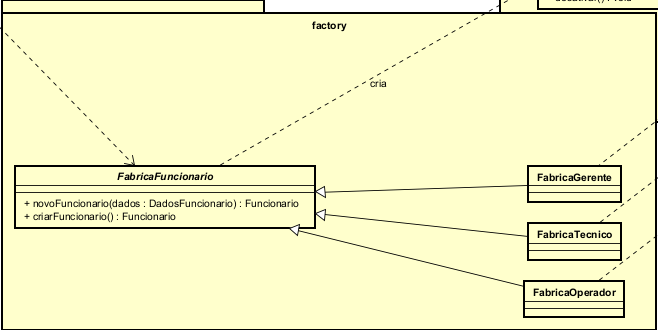
\includegraphics[width=0.8\textwidth]{Imagens/fabrica.png}
        \captionof{figure}{\label{fig:diagramaFactory}Diagrama de Classes - Padrão Factory Method}
\end{center}

\newpage

% ==================================================================
\section{Padrão Facade (Estrutural)}

\subsection{Problema identificado}
O fluxo de abertura e tramitação de uma falha envolve coordenar vários objetos:
criar a \texttt{Falha}, aplicar a estratégia de prioridade, registrar
\texttt{Evidencia} e \texttt{Diagnostico}, vincular a \texttt{Maquina} e
verificar o \texttt{AcordoNivelServico}. Exigir que o cliente
(controlador/interface) orquestrasse tudo isso o acoplava às entranhas do
subsistema.

\subsection{Solução proposta}
Criou-se a \texttt{FacadeGestaoFalha}, que expõe operações de alto nível
(\texttt{abrirFalha}, \texttt{aprovarFalha}, \texttt{atenderFalha},
\texttt{encerrarFalha}) e esconde a orquestração interna entre as diversas
classes do domínio.

\subsection{Justificativa técnica e por que usar}
O padrão Facade fornece uma interface unificada e simplificada para um conjunto
de interfaces de um subsistema. É adequado quando se deseja reduzir o
acoplamento do cliente com a complexidade interna. A fachada é também o ponto
natural de integração dos demais padrões: ela cria a \texttt{Falha}, escolhe a
\textit{Strategy}, registra os \textit{Observers} e utiliza a \textit{Factory}.

\subsection{Impacto arquitetural}
O cliente passa a depender de uma única classe de entrada, e não de toda a teia
de objetos do domínio. Isso melhora a legibilidade, facilita testes de fluxo e
isola futuras mudanças internas do subsistema.

\subsection{Vantagens e limitações}
\begin{itemize}[leftmargin=*]
    \item \textbf{Vantagens:} reduz o acoplamento do cliente; centraliza a
    orquestração; oferece um ponto único e estável de acesso.
    \item \textbf{Limitações:} pode evoluir para uma classe ``deus'' se acumular
    responsabilidades em excesso; adiciona uma camada de indireção.
\end{itemize}

\subsection{Trecho do diagrama de classes}
\begin{center}
        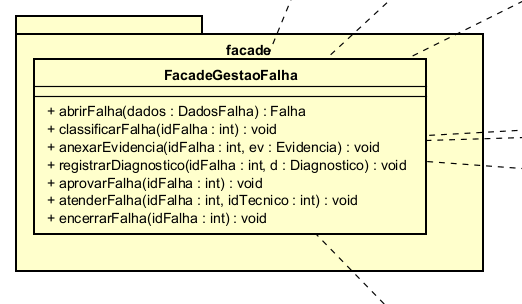
\includegraphics[width=0.8\textwidth]{Imagens/facade.png}
        \captionof{figure}{\label{fig:diagramaFacade}Diagrama de Classes - Padrão Facade}
\end{center}

\newpage



% ==================================================================
\section{Conclusão}

A aplicação dos cinco padrões transformou um diagrama com forte configuração de
responsabilidades em uma arquitetura coesa e de baixo acoplamento. Os padrões
\textbf{State} e \textbf{Strategy} retiraram a lógica de controle e de cálculo de
dentro da \texttt{Falha}; o \textbf{Observer} eliminou suas dependências de
saída; o \textbf{Factory Method} centralizou a criação de objetos; e o
\textbf{Facade} forneceu uma porta de entrada única para o subsistema. O conjunto
respeita princípios de projeto consagrados --- notadamente o \textit{Single
Responsibility Principle} e o \textit{Open/Closed Principle} --- resultando em um
sistema mais extensível, testável e manutenível, sem recorrer aos padrões
vedados pelo escopo (\textit{Abstract Factory}, \textit{Adapter} e
\textit{Decorator}).



\appendix  
\clearpage 



\end{document}